\chapter{Das Deep Learning Modell}\label{ch7}
\section{Analyse der Technologie}
\textit{TensorFlow} ist eine Bibliothek, mit der Deep Learning in Python durchgeführt werden kann. Es wurde im Jahr 2015 von Google Open Source gemacht. Mit TensorFlow werden die Daten als \enquote{Tensoren} dargestellt und fließen durch Schichten. Dieses ermöglicht die Inferenz und das Training in maschinellen Lernmodellen. Ein \textit{Tensor} ist ein multidimensionales Array. In neuronalen Netzen und beim Deep Learning wird jedes Datenelement und jedes Berechnungsergebnis als Tensor dargestellt, z.B. kann ein Graustufenbild als 2-dimensionales Array dargestellt werden oder ein Farbbild als 3-dimensionales Array. Der Tensor kann unterschiedliche Datentypen haben (z. B. float32 oder int32). Neben dem Typen eines Tensors gibt es die zweite Eigenschaft, die Form eines Tensors. Die Form eines Tensors gibt die Größe des Tensors entlang aller seiner Abmessungen an. Beispiel: Ein 2-dimensionales Tensor hat die Form (128, 256). Ein Tensor kann unabhängig von den ursprünglichen Daten in ein sogenanntes Layer eingespeist werden, welches nur danach schaut, welcher Datentyp und Form der Tensor hat. Tensoren sind also eine Art Container die Daten organisieren und dafür verwendet werden können, dass diese parallel verarbeitet werden können \cite[27]{cai2020deep}.


\begin{lstlisting}[language=Python,caption=Beispiel eines Tensors in TensorFlow, label={Label4}]
import tensorflow as tf


rank_2_tensor = tf.constant([[1, 2],
                             [3, 4],
                             [5, 6]], dtype=tf.float16)
\end{lstlisting}

Um den zweiten Ausdruck in \enquote{TensorFlow} zu verstehen, muss der Tensor als eine Art \enquote{Flüssigkeit} vorgestellt werden, welches die Daten trägt. In TensorFlow fließt es durch ein Diagramm - eine Datenstruktur, die aus miteinander verbundenen mathematischen Operationen (Knoten genannt) bestehen. Wie Abbildung~\ref{tnflayers} zeigt, kann der Knoten aufeinanderfolgende Schichten in einem neuronalen Netzwerk sein. Jedes der Knoten nimmt Tensoren als Eingabe und erzeugt Tensoren als Ausgabe. Die \enquote{Flüssigkeit} wird in verschiedene Formen und Werte umgewandelt, wenn sie durch das TensorFlow-Diagramm \enquote{fließt}. Dies entspricht der Transformation, d.h. dem Kern dessen, was neuronale Netze tun. Mit TensorFlow können Ingenieure für maschinelles Lernen, alle Arten von neuronalen Netzen schreiben, von flachen bis zu sehr tiefen Netzen \cite[27-28]{cai2020deep}.

 \begin{figure}[H]
     \centering
     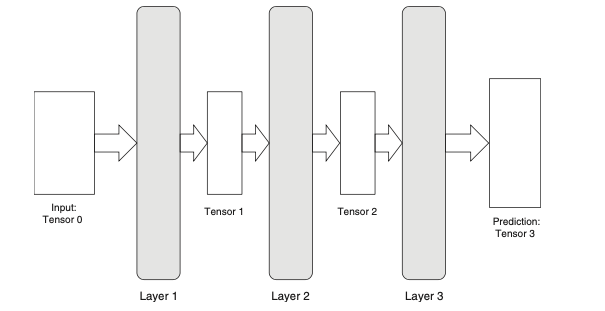
\includegraphics[width=13cm]{kapitel5/tflayers.png}
     \caption[Die Darstellung eines Deep Learning Modells in TensorFlow]{Die Darstellung eines Deep Learning Modells in TensorFlow - Die Tensoren fließen durch jede Schicht im Modell durch. Abbildung aus \cite[28]{cai2020deep}.}
     \label{Kap5:tnflayers}
 \end{figure}


Im Kern wurde TensorFlow sehr allgemein und flexibel konzipiert: Die Operationen können beliebige genau definierte mathematische Funktionen sein, nicht nur Schichten neuronaler Netze. Dies können beispielsweise mathematische Operationen auf niedriger Ebene sein, beispielsweise das Addieren und Multiplizieren von zwei Tensoren - die Art von Operationen, die innerhalb einer neuronalen Netzwerkschicht stattfinden. Dies gibt Deep-Learning-Ingenieuren und Forschern die Möglichkeit, beliebige und neuartige Operationen für Deep-Learning zu definieren. Für einen großen Teil der Deep-Learning-Praktiker ist die Manipulation solcher Operationen auf niedriger Ebene jedoch schwieriger als es sich lohnt. Dies führt zu aufgeblähtem und fehleranfälligerem Code und längeren Entwicklungszyklen. Die meisten Deep-Learning-Ingenieure verwenden eine Handvoll fester Schichttypen (z. B. Faltung, Pooling oder Dichte Schichten). In seltenen Fällen müssen neue Ebenentypen erstellt werden. Hier ist die \enquote{LEGO-Analogie} angebracht. Bei LEGOs gibt es nur wenige Blocktypen. \enquote{LEGO-Entwickler} müssen nicht darüber nachdenken, was nötig ist, um einen LEGO Block zu erstellen \cite[28]{cai2020deep}. 


In der Welt von TensorFlow ist das LEGO-Äquivalent die High-Level-API namens \textit{Keras}. Keras bietet eine Reihe der am häufigsten verwendeten Arten von neuronalen Netzwerkschichten mit jeweils konfigurierbaren Parametern. Außerdem können Benutzer die Schichten miteinander verbinden, um neuronale Netze zu bilden. Darüber hinaus enthält Keras auch APIs für:

\begin{itemize}
     \item Festlegen, wie das neuronale Netzwerk trainiert werden soll (Verlustfunktionen, Metriken und Optimierer)
     \item Daten einspeisen, um das neuronale Netzwerk zu trainieren oder auszuwerten oder das Modell zur Inferenz zu verwenden
     \item Überwachung des laufenden Trainingsprozesses
     \item Modelle speichern und laden
     \item Plotten der Architektur und von Modellen \cite[29]{cai2020deep}.
 \end{itemize}





Es gab jedoch ein Problem: Es war nicht möglich, TensorFlow- oder Keras-Modelle in JavaScript oder direkt im Webbrowser auszuführen. Um Deep-Learning-Modelle im Browser bereitzustellen, musste dies über HTTP-Requests an einen Backend-Server getan werden. \textit{TensorFlow.js} löst dieses Problem. Die JavaScript-API hat eine Keras-ähnliche High-Level-API welches auf dem Low-Level-Kern erstellt wurde, die es Benutzern erheblich erleichtert, Deep-Learning-Modelle in der JavaScript-Bibliothek zu definieren, zu trainieren und auszuführen. Um die Interoperabilität weiter zu verbessern, wurden Konverter erstellt, mit denen TensorFlow.js aus TensorFlow und Keras gespeicherte Modelle importieren und Modelle in diese exportieren kann \cite[29]{cai2020deep}.


\textit{Google Colab} ist ein kostenloser Cloud-Dienst auf Basis von Jupyter Notebooks, der GPU unterstützt. Dies ist nicht nur ein Tool zur Verbesserung der Codierungsfähigkeiten, sondern ermöglicht es auch absolut jedem, Deep-Learning-Anwendungen mit gängigen Bibliotheken wie PyTorch, TensorFlow, Keras und OpenCV zu entwickeln. Dabei wird die Hardware von Google über Cloud-Computer frei angeboten, sodass diese Kapazitäten zum Training von Deep Learning Modellen verwendet werden können. 

 \begin{figure}[H]
     \centering
     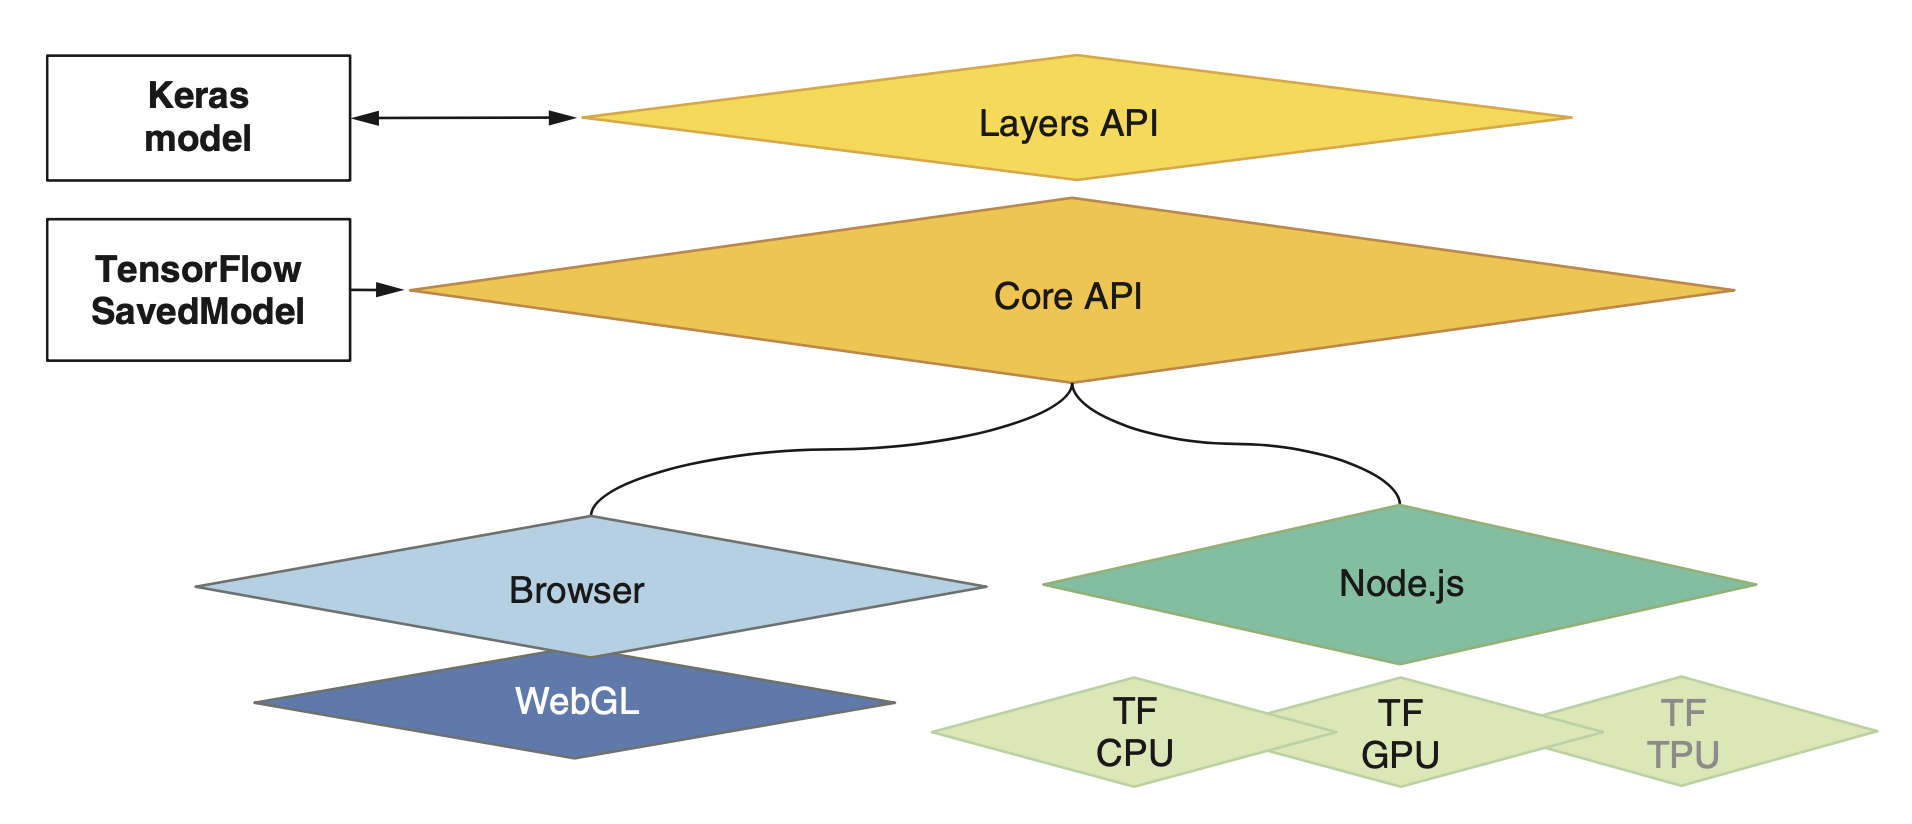
\includegraphics[width=12cm]{kapitel5/tfjsarch.png}
     \caption[Die Architektur von TensorFlow.js]{Die Architektur von TensorFlow.js - Abbildung zeigt die Verhältnisse zwischen der Python API von TensorFlow und Keras mit TensorFlow.js. Entnommen aus \cite[30]{cai2020deep}}
     \label{Kap5:tfjsarch}
 \end{figure}
 


\section{Vorverarbeitung}
Beim Vorverarbeitung (Preprocessing) der Daten sollte der Text zunächst in Einbettungen (Vektoren) umgewandelt werden, sodass ein Training erfolgen kann. Bei der Erstellung des Datensatzes wurden die Titel weitestgehend \enquote{gesäubert}. Bei einigen Schlagzeilen waren neben dem Titel auch Namen der Seite vorhanden, diese wurden entfernt. Jedoch sollte der Text, wenn noch nicht erfolgt, in Kleinbuchstaben umgewandelt werden. Die Leerzeichen nach und vor dem jeweiligen Satzzeichen sollten getrennt werden. Da bei Clickbaits Satzzeichen wie Fragezeichen oder Ausrufezeichen eine wichtige Bedeutung haben, werden diese nicht vollständig entfernt und in den Vokabular aufgenommen. Es werden also alle Satzzeichen außer Fragezeichen, Ausrufezeichen und Punkt entfernt. Stoppwörter bieten normalerweise keine große Relevanz, sind hier jedoch auch bedeutsam, z.B. Präpositionen. Stoppwörter werden nicht entfernt.

Beim Preprocessing wird der Datensatz in zwei Teile geschnitten, dem Trainingssatz und des Testsatz. Es ist üblich dieses Teilung in einer Ratio von 0.8/0.2 auszuführen. Das Ziel ist es vorherzusagen, ob eine bestimmte Schlagzeile Clickbait ist oder nicht. Das Modell muss also später vorhersagen mit neuen Texten treffen. Um den Erfolg des Modells messen zu können wird ein Teil des Datensatzes also getrennt von dem Trainingsdatensatz. Dieser kleinere Teil dient zur Überprüfung des Modells nach dem Training. Diese \enquote{neue} Daten werden dann dem Modell nach dem Trainings gezeigt, um zu sehen wie gut es performt. Aus diesem Grund ist beim Preprocessing der Datensatz in Trainingssatz und Testsatz aufzuteilen. In der Funktion aus Listing~\ref{TrainTestFunc} wird der Datensatz aus einer CSV-Datei gelesen und mittels Pandas in ein Dataframe umgewandelt. Es werden zufällig 80\% der Titel \enquote{maskiert} und entsprechend aufgeteilt und als Tupel zurückgegeben. Es entstehen somit ca. 16.000 Beispiele für das Training und 4.000 Beispiele für das Testen.

\begin{lstlisting}[language=Python,caption=Funktion für das Aufteilen des Datensatzes, label={TrainTestFunc}]
import pandas as pd
import numpy as np


def create_train_test(csv_file_path):
    dataframe_ = pd.read_csv(csv_file_path).drop_duplicates()
    msk = np.random.rand(len(dataframe_)) < 0.8
    train = dataframe_[msk]
    test = dataframe_[~msk]
    test.reset_index(drop=True)
    train.reset_index(drop=True)
    return train, test;
\end{lstlisting}

Im Listing~\ref{CleanFunct} werden die Buchstaben in Kleinbuchstaben umgewandelt. Mit dem regulären Ausdruck wird jedes Wort in Tokens umgewandelt. Um die Fragezeichen und Ausrufezeichen herum werden Leerzeichen gesetzt, um diese vom jeweiligen Wort zu trennen und auch als Token zu erhalten. Zahlen werden behalten.

\begin{lstlisting}[language=Python,caption=Die Preprocessing-Funktion, label={CleanFunct}]
import re


def text_cleaner(text):
    newtext = re.sub(r"[^A-Za-z?!.0-9üäöß]+", " ", text)
    newtext = re.sub("([!?])", r" \1 ", newtext)
    newtext = re.sub("\s{2,}", " ", newtext)
    return newtext.lower()
    
    
train["Title"] = train["Title"].apply(lambda x: text_cleaner(x))
test["Title"] = test["Title"].apply(lambda x: text_cleaner(x))
\end{lstlisting}

\section{Das Erstellen eines Vokabulars} \label{vocSec}


Es ist wichtig ein Vokabular bekannter Wörter zu definieren, wenn One-Hot-Encoding oder ein Worteinbettungen verwendet werden. Je mehr Wörter vorhanden sind, desto größer ist die Darstellung von Dokumenten. Daher ist es wichtig, die Wörter nur auf diejenigen zu beschränken, von denen angenommen wird, dass sie vorhersagbar sind. Dies ist im Voraus schwierig. Es ist oft wichtig, verschiedene Hypothesen zum Aufbau eines nützlichen Vokabulars zu testen. Aus dem vorherigen Abschnitt wurde die Interpunktion entfernt. Zahlen wurden nicht entfernt und auch Stoppwörter sind dem Datensatz erhalten geblieben. Es kann also aus allen Schlagzeilen eine Reihe aller bekannten Wörter ermittelt werden. Jedes Element im Vokabular wird als Zahl dargestellt. Es handelt sich also um eine Wörterbuch Zuordnung von Wörtern und deren Index. Somit kann das Wort auf eine einfache Weise aktualisiert und abgefragt werden.

Keras bietet eine Klasse namens \texttt{Tokeniser} (siehe Listing \ref{TokenizerFunc}) welches diesem Zwecke dient. Diese Klasse ermöglicht die Vektorisierung von Textkorpora, indem jedes Token entweder in eine Folge von Ganzzahlen (jede Ganzzahl ist der Index eines Tokens in einem Wörterbuch) oder in einen Vektor umgewandelt wird. Die Methode \texttt{fit\_on\_texts} dieser Klasse aktualisiert den internen Wortschatz anhand einer Liste. Um den Text in eine Folge von ganzen Zahlen umzuwandeln ist das Ausführen der Methode \texttt{fit\_on\_texts} zwingend erforderlich. Dann können mit der Methode \texttt{texts\_to\_sequences}, die Wörter die der Tokeniser am häufigsten gesehen hat ermittelt werden. Der nächste Schritt ist das Padding. Mit der Methode \texttt{pad\_sequences} kann eine Liste von Sequenzen mit einer bestimmten Länge in ein 2-dimensionales Numpy-Array umgewandelt werden. Sequenzen die länger als die angegebene maximale Länge haben, werden abgeschnitten, damit sie der gewünschten Länge entsprechen. Sequenzen die kürzer sind wiederum, werden mit einer Null aufgefüllt, bis sie dem maximalen Wert entsprechen. Das Vorfüllen oder Entfernen von Werten am Anfang der Sequenz ist die Standardeinstellung. Im aktuellen Datensatz haben die Titel  eine maximale Tokenlänge von 21. Die maximale Länge wird auf 40 Tokens gesetzt. Es wird also nachher erlaubt, eine Abfrage mit maximal 40 Tokens durchzuführen. Es ist nicht zu erwarten, dass eine Schlagzeile mehr als 40 Tokens hat. Der Tokeniser gibt somit z.B. für den Titel \enquote{die 10 besten apps für mädchen} einen Array der Länge 40 zurück, wobei die ersten 34 Werte eine Null enthalten und die restlichen 6 eine bestimmte Zahl, welches den Index des Wortes darstellt.



\begin{lstlisting}[language=Python,caption=Die Tokeniser-Funktion, label={TokenizerFunc}]
from keras.preprocessing.text import Tokenizer
from keras.preprocessing.sequence import pad_sequences


def tokenize_text(train_df, test_df, max_l):
    tokenizer = Tokenizer(filters='"#$%&()*+-/:;<=@[\\]^_`{|}~\t\n')
    tokenizer.fit_on_texts(train_df)
    vocab_size = len(tokenizer.word_index) + 1
    tokenized_text_train = pad_sequences(
        tokenizer.texts_to_sequences(train_df), maxlen=max_l)
    tokenized_text_test = pad_sequences(
        tokenizer.texts_to_sequences(test_df), maxlen=max_l)
    return {"tokenized_text_train": tokenized_text_train, "tokenized_text_test": tokenized_text_test, "vocab_size": vocab_size, "tokenizer": tokenizer}
\end{lstlisting}


Eine Worteinbettung ist eine Möglichkeit, Text darzustellen, bei der jedes Wort im Vokabular durch einen reellen Vektor in einem hochdimensionalen Raum ersetzt wird. Die Vektoren werden so gelernt, dass Wörter mit ähnlichen Bedeutungen eine ähnliche Darstellung im Vektorraum haben (nahe im Vektorraum). Dies ist eine aussagekräftigere Darstellung für Text als klassische Darstellungen, bei denen Beziehungen zwischen Wörtern oder Tokens ignoriert oder in Bigram- und Trigramm-Ansätzen erzwungen werden. Die Vektordarstellung für Wörter kann während des Trainings des neuronalen Netzwerks gelernt werden. Dieses kann in der Keras Deep Learning-Bibliothek mithilfe der Einbettungsebene ausgeführt werden. Alternativ können auch vortrainierte Einbettungen wie Word2Vec verwendet werden, die auf eine große Menge an Daten vortrainiert und für neue Aufgaben verwendet werden können. In dieser Arbeit wird die erste Alternative der Worteinbettung verwendet.


Die Keras-Einbettungsschicht erfordert Ganzzahl Eingaben, bei denen jede Ganzzahl einem einzelnen Token zugeordnet ist, das eine bestimmte reelle Vektordarstellung innerhalb der Einbettung repräsentiert. Diese Vektoren sind zu Beginn des Trainings zufällig, gewinnen jedoch während des Trainings für das Netzwerk an Bedeutung. Durch die Funktionen aus Listing~\ref{CleanFunct} und Listing~\ref{TokenizerFunc} wurde das Encoding bestimmt, also der Text in ein passendes Format gebracht. Schließlich werden die Klassenbezeichnungen für den Trainingsdatensatz und Testdatensatz definieren, die für das überwachte neuronale Netzwerkmodell erforderlich sind. Die Daten werden zuletzt in ein TensorFlow dataset umgewandelt, um sie leichter in Keras einzuspeisen. Somit entsteht ein Datensatz für das Training, mit einem Wortschatz  von ca. 23.000 Vokabeln und einem erwarteten maximalen Eingang von 30 Tokens. Die Daten wurden in Trainingssatz und Testsatz aufgeteilt. Mit der Funktion aus Listing~\ref{LabelFunc} werden die Labels \textit{Clickbait 0} und  \textit{News 1} in ein Array umgewandelt. Im Listing \ref{DataSet} wird der Datensatz in ein TensorFlow Datensatz umgewandelt. Dadurch können die Daten direkt in ein Modell eingespeist werden. In diese Funktion gehen auch die labels \textit{y} und \textit{y\_test} hinein. 

\begin{lstlisting}[language=Python,caption=Die Label-Funktion, label={LabelFunc}]
def create_labels(train_data, test_data):
    encoded_labels = preprocessing.LabelEncoder()
    y = encoded_labels.fit_transform(train_data["label"])
    y = to_categorical(y)
    y_test = encoded_labels.transform(test["label"])
    y_test = to_categorical(y_test)
    return y, y_test;

y, y_test = create_labels(train, test)
\end{lstlisting}

\begin{lstlisting}[language=Python,caption=Die Dataset Erstellung, label={DataSet}]
import tensorflow_datasets as tfds

train_dataset = tf.data.Dataset.from_tensor_slices((tokenized_text_train, y))
test_dataset = tf.data.Dataset.from_tensor_slices((tokenized_text_test, y_test))
\end{lstlisting}





\section{Die Modell Architektur}



In Listing~\ref{BuildModel} wird ein sequentielles Modell erstellt. Diesem Modell kann durch die Methode \texttt{add} jeweils eine Schicht angehängt werden, und Keras arbeitet dieses nacheinander ab. Die API von Keras wird verwendet um das Modell zusammen zu bauen. Die Definitionen der einzelnen Methoden mit der das Modell gebaut und trainiert wurde, sind aus der Dokumentation von Google \citep{google1} entnommen. Dort werden viele Begriffe, die im Zusammenhang mit dem bauen und trainieren eines Deep Learning oder Machine Learning Modells stehen, erklärt. Aus diesem Grund wird in den nächsten zwei Abschnitten auf diese Quelle verwiesen.

\begin{lstlisting}[language=Python,caption=Das Bilden des Models, label={BuildModel}]
from tensorflow.keras.models import Sequential
from tensorflow.keras.layers import Conv1D, MaxPool1D, Dropout, Dense, GlobalMaxPool1D, Embedding, Activation

def build_model(vocab_size, emb_dim, max_len, dropout_rate, learning_rate, n_labels):
    loss = tf.keras.losses.BinaryCrossentropy()
    metric = [tf.keras.metrics.BinaryAccuracy(name="accuracy")]
    opt = tf.keras.optimizers.Adam(learning_rate=learning_rate)

    model = Sequential([])
    model.add(
        Embedding(vocab_size, output_dim=emb_dim, input_length=max_len))
    model.add(Dropout(dropout_rate))
    model.add(Conv1D(filters=32, kernel_size=8,
                           activation="relu", padding="same", strides=1))
    model.add(GlobalMaxPool1D())
    model.add(Dense(16, activation="relu"))
    model.add(Dense(n_labels, activation="softmax"))
    model.compile(loss=loss, metrics=metric, optimizer=opt)
    model.summary()
    return model
    
model = build_model(vocab_size=vocab_size, emb_dim=32, max_len=40, dropout_rate=0.3, learning_rate=0.00006, n_labels=len(labels))
\end{lstlisting}


Zunächst müssen einige Parameter festgelegt werden. Diese sind \texttt{loss} also die Verlustfunktion, \texttt{metric} also nach welchen Metriken das Modell bemessen werden soll und \texttt{opt} der \texttt{Optimizer} wodurch das Modell lernt. Da es sich um eine binäre Klassifikation handelt, ist hier die \texttt{BinaryCrossentropy} als Verlustfunktion ausgewählt worden. Selbes gilt für die \texttt{BinaryAccuracy}. Als Optimizer wurde \texttt{Adam} ausgewählt. Die Lernrate ist ein Skalar, mit dem ein Modell über einen Gradientenabstieg trainiert wird. Während jeder Iteration multipliziert der Gradientenabstiegsalgorithmus die Lernrate mit dem Gradienten. Das resultierende Produkt wird als Gradientenschritt bezeichnet. Die Lernrate ist ein wichtiger Hyperparameter. Ein Optimizer ist eine spezifische Implementierung des Gradientenabstiegsalgorithmus. Die Klasse von TensorFlow für Optimierer ist \texttt{tf.train.Optimizer}. Die Auswahl der Hyperparameter erfolgt durch das experimentieren und testen des Verfassers dieser Arbeit (siehe Listing \ref{BuildModel} Zeile 5-7).

Nachdem die Hyperparameter popularisiert wurden, wird dem Modell die erste Schicht zugeführt. Dieses ist die Einbettungsschicht. Die Worteinbettung sind eine Möglichkeit, ein Wort als Vektor darzustellen (ein 1-dimensionaler Tensor in TensorFlow). Durch Worteinbettungen können die Werte der Elemente des Vektors trainiert werden. Es muss also keine Regel angewendet werden, wie bei der One-Hot-Codierung und dessen Wort zu Index Zuordnung. Mit anderen Worten, wenn ein textorientiertes neuronales Netzwerk die Worteinbettung verwendet, werden die Einbettungsvektoren zu trainierbaren Gewichtungsparametern des Modells. Sie werden durch dieselbe Backpropagation-Regel wie alle anderen Gewichtungsparameter des Modells aktualisiert. Es gibt auch die Möglichkeit, eine vortrainierte Einbettungsschicht zu verwenden. Diese werden auf viel größere Mengen an Daten trainiert und können für vielseitige Zwecke verwendet werden, ohne dass von Grunde aus neu trainiert werden muss. In diese Fall trainiert das Modell die Einbettungen selbst, anstatt sich auf die vorab trainierten Einbettungen zu verlassen (siehe Listing \ref{BuildModel} Zeile 10-11).


Um das Modell vor Überanpassung zu schützen gibt es bestimmte Strategien, die angewendet werden können. Dieses sind sogenannte Regularisierungstrategien. Es kann als eine Art \enquote{Strafe} betrachtet werden, für die Komplexität des Modells und das nicht Vorhandensein an Daten. Da bei wenig Daten und hoher Komplexität das Modell nicht wirklich lernt, sondern sich den gegebenen wenigen Daten \enquote{über anpasst} können diese Strategien dagegen steuern (siehe Listing \ref{BuildModel} Zeile 12). Wenn Neuronen Muster in Trainingsdaten vorhersagen, indem sie sich fast ausschließlich auf Ausgaben bestimmter anderer Neuronen stützen, anstatt sich auf das Verhalten des Netzwerks als Ganzes zu verlassen, entsteht eine Anpassung. Wenn die Muster, die eine Anpassung verursachen, nicht in den Validierungsdaten vorhanden sind, weil es zu wenig Daten vorhanden sind etwa, führt dies zu einer Überanpassung. Die Dropout-Regularisierung reduziert die Anpassung, da Dropout sicherstellt, dass sich Neuronen nicht nur auf bestimmte andere Neuronen verlassen können. Die Dropout-Regularisierung entfernt eine zufällige Auswahl einer festen Anzahl von Einheiten in einer Netzwerkschicht für einen einzelnen Gradientenschritt. Je mehr Einheiten ausfielen, desto stärker war die Regularisierung.


Die \texttt{Conv1D}-Ebene (siehe Listing \ref{BuildModel} Zeile 13) wird verwendet um die Faltung durchzuführen. Eine CNN ist ein neuronales Netzwerk, in dem mindestens eine Schicht die Faltungsschicht ist. Ein typisches neuronales Faltungsnetzwerk besteht aus einer Kombination der von Faltungsschichten, Poolingschichten, und vollständig verbundene Schichten. Die Faltungsschicht hier ist eine eindimensionale Faltungsschicht. Bestimmte Muster aus dem Text werden hier erkannt (z.B. ob nach einem negativen Verb ein bestimmtes Wort auftaucht. In dem Beispiel gibt es 32 Filter. Beim maschinellen Lernen werden Faltungsfilter normalerweise mit Zufallszahlen gesetzt, und dann trainiert das Netzwerk die idealen Werte. Die \textit{kernel\_size} ist eine Zahl, die die Höhe des Faltungsfensters angibt. Zusätzlich zur eindimensionalen Faltungsschicht wird eine ebenfalls eindimensionale Poolingsschicht (siehe Listing \ref{BuildModel} Zeile 15) zugeführt.


Die \texttt{Dense}-Schichten (siehe Listing \ref{BuildModel} Zeile 16-17) sind verborgene Schichten, in der jeder Knoten mit jedem Knoten in der nachfolgenden verborgenen Schicht verbunden ist. Eine vollständig verbundene Schicht wird auch als dichte Schicht \enquote{dense layer} bezeichnet. Das erste der beiden Schichten im Modell hat 16 Einheiten und das zweite hat genau so viele Einheiten wie es Labels gibt (dieses Modell hat genau 2, da es 2 Klassen gibt). Die letzte Schicht ist somit die Ausgabeschicht und teilt die Vorhersage mit.


Mit der \texttt{compile}-Methode lässt sich das Modell bauen und die \texttt{summary}-Methode gibt eine Übersicht über das Modell (siehe Tabelle~\ref{modellBesch}).


\begin{table}[h]
    \caption{Beschreibung der Schichten des Modells}
    \label{modellBesch}
    \renewcommand{\arraystretch}{1.2}
    \centering
    \sffamily
    \begin{footnotesize}
        \begin{tabular}{l l l}
            \toprule
            \textbf{Layer (type)}                  & \textbf{Output Shape} & \textbf{Param \#} \\
            \midrule
            embedding (Embedding)  & (None, 40, 32) & 740384                \\
            dropout (Dropout)  & (None, 40, 32) &     0      \\
            conv1d (Conv1D)                  & (None, 40, 32)     &    8224     \\
            global\_max\_pooling1d (GlobalMaxPool1D)   & (None, 32)                    &     0   \\
            dense (Dense)    & (None, 16)     &  528      \\
            dense (Dense)   & (None, 2)     & 34                      \\
            \bottomrule
        \end{tabular}
    \end{footnotesize}
    \rmfamily
\end{table}

\section{Das Training}

Mit der Funktion \texttt{train\_model} aus Listing~\ref{TrainModel} lässt sich das Modell trainieren. Zunächst muss als Parameter angegeben werden, wie viele Trainingsepochen das Modell trainiert werden soll. Ein vollständiger Trainingsdurchlauf über den gesamten Datensatz, sodass jedes Beispiel einmal gesehen wurde wird als Epoche genannt. Die \texttt{batch\_size} sind die Anzahl der Beispiele in einer Epoche. Vor dem Training bietet sich die Möglichkeit, die Daten zu mischen, dieses erfolgt mit dem Parameter \textit{shuffle}. Analysen über das Training kann mit TensorBoard durchgeführt werden. TensorBoard bietet die Visualisierung und Werkzeuge, die für Experimente mit maschinellem Lernen erforderlich sind. Metriken wie Verlust und Genauigkeit können mit TensorBoard für jede Epoche dargestellt werden. Damit TensoBoard im späteren Verlauf verwendet werden kann, wird eine Callback-Funktion eingeführt, welches den Verlauf des Trainings in Logdateien speichert. Mit der \textit{fit}-Methode erfolgt das Training (siehe Listing~\ref{TrainModel}).


\begin{lstlisting}[language=Python,caption=Das Training des Models, label={TrainModel}]
import os
import datetime

def train_model(num_epochs, batch_size, train_ds, test_ds, model, shuffle):
    ds_train_encoded = train_ds.shuffle(shuffle).batch(batch_size)
    ds_test_encoded = test_ds.batch(batch_size)
    logdir = os.path.join(
        "logs", datetime.datetime.now().strftime("%Y%m%d-%H%M%S"))
    tensorboard_callback = tf.keras.callbacks.TensorBoard(
        logdir, histogram_freq=1)
    model.fit(ds_train_encoded, epochs=num_epochs,
              validation_data=ds_test_encoded, callbacks=[tensorboard_callback])
    
train_model(num_epochs=7, batch_size=32, train_ds=train_dataset, test_ds=test_dataset, model=model, shuffle=1000)
\end{lstlisting}





\section{Evaluation}\label{evaSec}

Das Kreuzvalidierungsverfahren ist ein Mechanismus zum Testen, dafür um zu sehen, wie gut sich ein Modell auf neue Daten verallgemeinern lässt. Das Modell wird mit neuen Daten, welche dem Trainingsdatensatz zurückgehalten wurden, getestet. Mit der Bibliothek \enquote{sklearn} können mit der Methode \texttt{classification\_report} ein Testbericht mit den wichtigsten Klassifizierungsmetriken erstellt werden. Dieser Report gibt Auskunft über bestimmte Metriken, mit der das Performance des Modells auf den vorhandenen Daten gemessen werden kann. 

\begin{lstlisting}[language=Python,caption=Das Evaluieren des Models, label={TrainModel}]
import numpy as np
from keras.utils import to_categorical
from sklearn.metrics import classification_report

y_pred = to_categorical(np.argmax(
    model.predict(tokenized_text_test), axis=1))

print(classification_report(y_test, y_pred, target_names=labels.values(), digits=4))
\end{lstlisting}



\begin{table}[h]
    \caption{Die Ergebnisse der Evaluation des Modells}
    \label{eval1}
    \renewcommand{\arraystretch}{1.2}
    \centering
    \sffamily
    \begin{footnotesize}
        \begin{tabular}{l l l l l}
            \toprule
                           & \textbf{precision} & \textbf{recall} & \textbf{f1-score} & \textbf{support} \\
            \textbf{Clickbaits} & 0.9775                  & 0.9589                 & 0.9681                & 1993          \\
            \textbf{News}  & 0.9590                 & 0.9776                & 0.9682               & 1961                     \\
            \bottomrule
        \end{tabular}
    \end{footnotesize}
    \rmfamily
\end{table}

\begin{figure}[H]
    \centering
    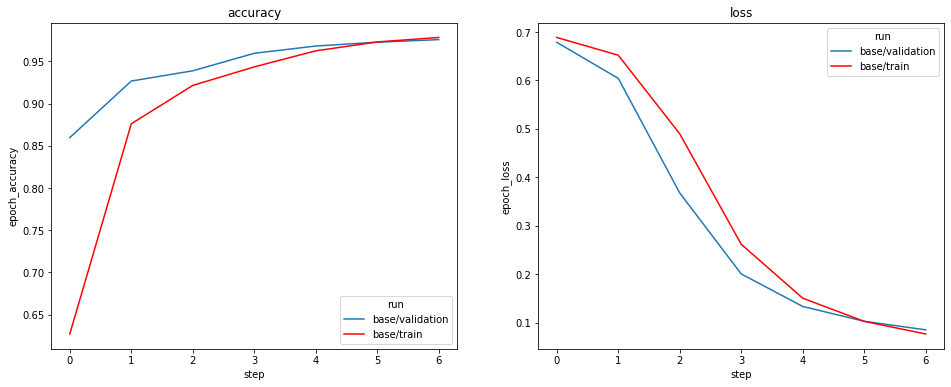
\includegraphics[width=15cm]{kapitel5/basemodel.png}
    \caption[Vergleich der Trainingsdaten mit den Validierungsdaten]{Blau: Validierungsdaten. Rot: Trainingsdaten. Links: Die Genauigkeit nimmt mit jeder Epoche zu und beide Kurven nähern sich an bis sie sich in der 7. Epoche treffen. Rechts: Die Verlustfunktionen beider Daten werden dargestellt. Die Graphen treffen sich erst in der 5. Epoche. Hier liegt kein optimaler \enquote{Fit} vor, da beide Graphen meistens auseinander liegen.}
    \label{Kap5:Val}
\end{figure}


Um zu das Modell auch praktisch zu testen und zu sehen wie es in der Realität performt sollen dem Modell neue Anfragen gesendet werden. Nachdem das Modell diese Anfragen beantwortet, kann gesehen werden wo es gut abschneidet und und wo nicht und potenzielle Schwachstellen festgelegt werden. Natürlich wird das Modell in Wirklichkeit nicht so gut performen wie in der Tabelle \ref{eval1}. Die Realität bietet einen viel größeren \enquote{Datensatz} und viel komplexere Anfragen. Es ist unmöglich, ein Modell zu entwickeln, welches auf alle Gegebenheiten trainiert wird. Zum Abschluss dieses Abschnittes sollen einige \enquote{Schwachstellen} dieses Modells mittels praktischer Anwendung dargestellt werden. Es ist zu erwarten, dass das Modell \enquote{offensichtliche Clickbaits} gut erkennt, jedoch ist zu beantworten, wie es sich \enquote{mehrdeutigen Fällen} verhält. 



\begin{table}[h]
    \caption{Vorhersagen des Modells für neue Schlagzeilen}
    \label{PredictNewTab}
    \renewcommand{\arraystretch}{1.2}
    \centering
    \sffamily
    \begin{footnotesize}
        \begin{tabular}{l l}
            \toprule
            \textbf{Schlagzeile}                  & \textbf{Vorhersage} \\
            \midrule
            Die 10 lustigsten Bilder von Katzen! & Clickbait \\
            Diese Rezepte solltest du nicht verpassen!  & Clickbait    \\
            Aus diesem Grund sollten Sie ihr Smartphone während des Schlafens ausschalten                  & Clickbait       \\
            13 Dinge, die Sie garantiert noch nicht über ihr Smartphone wussten   & Clickbait                   \\
            Sondersitzung des Kabinetts - Bayern ruft erneut Katastrophenfall aus   & News        \\
            Russland verschärft Ton im Pipeline-Streit  & News                     \\
            Nordkorea präsentiert offenbar modernisierte Raketentypen & News \\
            „Wandelnde Arzneimittelwerbung“ als Kanzlerkandidat? & News \\
            Corona im News-Ticker: RKI meldet über 2 Mio. Infektionen - droht Mega-Lockdown? & Clickbait \\
            Die 7 besten Tageslinsen 2021 im Vergleich & Clickbait \\
            Er hatte alles – nur ein Erbe fehlte ihm: Zum Tod von Modegenie Pierre Cardin & Clickbait \\
            „Pass mal auf“: Lanz fragt nach Tempolimit 130, Merz knallt ihm einen vor den Latz & News \\
            Trump ist ein Politverbrecher wie Putin oder Erdoğan & Clickbait \\
            Wie Kinder die Corona-Pandemie beeinflussen & Clickbait \\
            Was steht in den Impfstoff-Verträgen? & Clickbait \\
            \bottomrule
        \end{tabular}
    \end{footnotesize}
    \rmfamily
\end{table}

In der Tabelle~\ref{PredictNewTab} sind die Ergebnisse des Experiments zu sehen. Es lassen sich bestimmte Muster erkennen. Offensichtliche Clickbaits und Nachrichten (die ersten 8 Schlagzeilen) werden erkannt. In diesen 8 Schlagzeilen haben Clickbaits die Eigenschaft, eine Zahl zu beinhalten und relativ kurze Wortlängen zu haben. Außerdem ist deutlich zu sehen, dass bei den Nicht-Clickbaits Nachrichten, es sich um Internationale Themen handelt und lange Wörter wie \enquote{Kanzlerkandidat} oder \enquote{Arzneimittelwerbung} vorhanden sind.

Das Modell kann aber auch falsch Alarm schlagen. Wie im Beispiel \enquote{Corona im News-Ticker: RKI meldet über 2 Mio. Infektionen - droht Mega-Lockdown?}, zwar ist hier ein Wort \enquote{Mega} welches ein oft in Clickbaits vorkommendes Wort ist und auch eine Zahl \enquote{2} enthalten, ebenfalls wird eine Frage gestellt. Das Modell kann aber nicht erkennen, bzw. weiß nicht, dass diese Mittel (das Stellen einer Frage, verwenden von Zahlen usw.) auch in konventionellen Nachrichten verwendet werden. Hier wird deutlich, dass alleine die Klassifizierung des Titels der Nachricht, auch zu falschen Ergebnissen führen kann. Es sollte ebenfalls der Inhalt der Nachricht überprüft und aus dem Zusammenhang beider Ergebnisse eine Vorhersage gemacht werden. 
\section{Experimente}
Das Modell aus der Tabelle \ref{modellBesch} erzeugt keinen perfekten Fit. Durch Experimente soll versucht werden dieses Problem zu beheben. Lässt sich durch die Änderung einiger Hyperparameter, dieses Problem beheben? In diesem Abschnitt werden einige Experimente mit den Hyperparametern gemacht und das Modell zum Ursprünglichen Modell aus Tabelle \ref{modellBesch} verglichen. Wie im Abschnitt~\ref{overundersec} beschrieben ist die Über- bzw. Unteranpassung zu vermeiden. Zwar gibt es Strategien wie im Abschnitt~\ref{regSec} definiert, aber auch die Anpassung der Hyperparameter wie die Lernrate können Auswirkungen auf die Über- oder Unteranpassung haben. Die Experimente sollen untersuchen, ob und wie sich das Modell ändert. Das Modell aus Tabelle~\ref{modellBesch} hat 32 Einbettungsdimensionen. Die Lernrate beträgt 0.00006 und sie hat eine Dropout-Rate von 0.35. Ziel ist es zu sehen, ob das Modell besser performt oder nicht und dabei nicht eine Überanpassung entsteht. 

\paragraph{Die Veränderung der Einbettungsdimension}
Die Einbettungsdimension ist der Parameter, der über die Dimensionalität der Einbettung entscheidet. Je größer diese Dimension ist, desto mehr Parameter sollten entstehen, da das Modell diese Einbettungen lernen muss. Somit würde vom Volumen her ein größeres Modell entstehen. Dieser Parameter wird von 32 auf 320 gesetzt. Alle anderen Parameter werden nicht verändert. An der Performance ändert sich wenig (siehe Tabelle~\ref{eval32}) jedoch entsteht eine Überanpassung ab der 3. Epoche des Trainings (siehe Abbildung~\ref{32embdpic}).

\begin{table}[h]
    \caption{Die Ergebnisse des Modells mit 320 Einbettungsdimensionen}
    \label{eval32}
    \renewcommand{\arraystretch}{1.2}
    \centering
    \sffamily
    \begin{footnotesize}
        \begin{tabular}{l l l l l}
            \toprule
                           & \textbf{precision} & \textbf{recall} & \textbf{f1-score} & \textbf{support} \\
            \textbf{Clickbaits} & 0.9761                  & 0.9867                 & 0.9814                & 1948          \\
            \textbf{News}  & 0.9869                 & 0.9766                & 0.9817               & 2009                     \\
            \bottomrule
        \end{tabular}
    \end{footnotesize}
    \rmfamily
\end{table}

\begin{figure}[H]
    \centering
    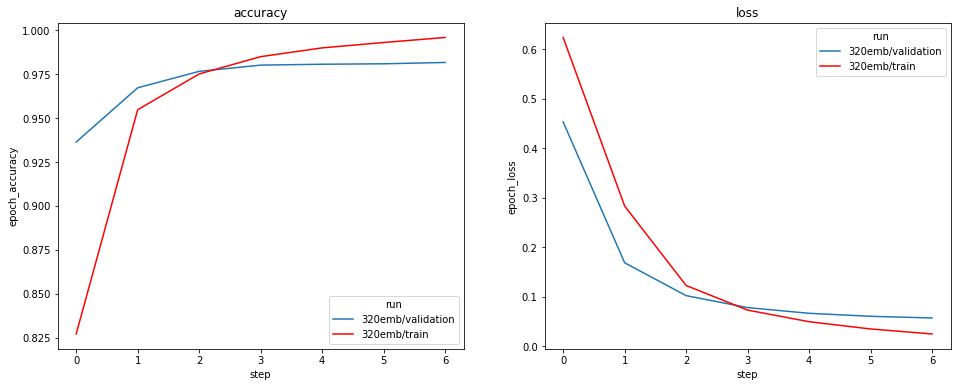
\includegraphics[width=15cm]{kapitel5/320embd.png}
    \caption[Auswirkung der Einbettungsdimensionen]{Ab der 3. Epoche findet eine Überanpassung statt.}
    \label{32embdpic}
\end{figure}

\paragraph{Die Veränderung der Der Lernrate von 0.00006 auf 0.0006}
Im Abschnitt~\ref{learnsection} wurde die Bedeutung der Lernrate im Deep Learning vorgestellt. Durch die verzehnfachung der Lernrate (von 0.00006 auf 0.0006) lernt das Modell mit einer höheren Rate und es ist in der Abbildung~\ref{learnpic} deutlich zu sehen, dass eine Überanpassung herrscht. Das Modell hat bereits nach der ersten Epoche das meiste gelernt.

\begin{table}[h]
    \caption{Die Ergebnisse der Evaluation des Modells mit einer Lernrate von 0.0006}
    \label{evallearn}
    \renewcommand{\arraystretch}{1.2}
    \centering
    \sffamily
    \begin{footnotesize}
        \begin{tabular}{l l l l l}
            \toprule
                           & \textbf{precision} & \textbf{recall} & \textbf{f1-score} & \textbf{support} \\
            \textbf{Clickbaits} & 0.9778                 & 0.9933                 & 0.9855                & 1948          \\
            \textbf{News}  & 0.9934                 & 0.9781                & 0.9857               & 2009                     \\
            \bottomrule
        \end{tabular}
    \end{footnotesize}
    \rmfamily
\end{table}

\begin{figure}[H]
    \centering
    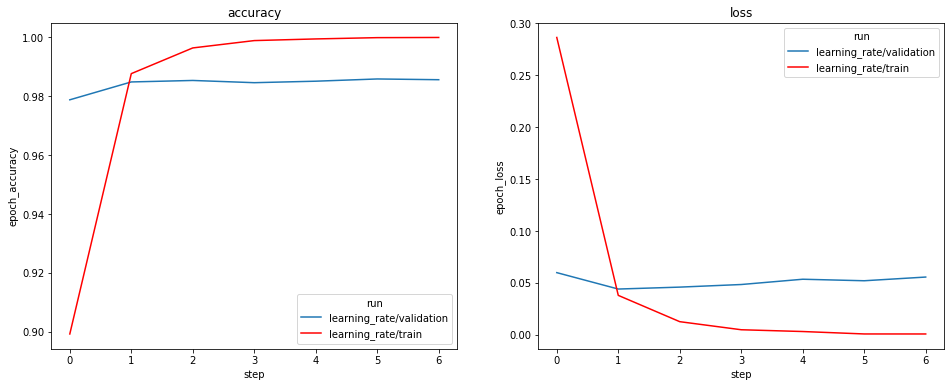
\includegraphics[width=15cm]{kapitel5/learningrate.png}
    \caption[Auswirkung der Lernrate]{Es ist zu sehen, wie das Modell in der ersten Epoche das meiste gelernt hat und sich danach nur noch dem Modell anpasst.}
    \label{learnpic}
\end{figure}

\paragraph{Das Hinzufügen von zusätzlichen Schichten}
Dem Modell aus Tabelle~\ref{modellBesch} werden zusätzliche Conv1D-Schichten hinzugefügt. Zusätzlich werden dem Modell 256 statt 32 Einbettungsdimensionen hinzugefügt. Die Dropout-Rate wird auf 0.1 runter gesetzt, da dieses Modell mehr Schichten dieser Art besitzt. Die Lernrate bleibt unverändert. Die Schichten werden nach der Beschreibung aus der Tabelle~\ref{modellBesch2} angepasst. Auch hier findet ein \enquote{schnelles Lernen} statt, wie in Abbildung~\ref{extrlayerspic} dargestellt. Es findet auch hier eine Überanpassung statt. Das Modell hat zusätzliche Faltungsschichten (siehe Tabelle~\ref{modellBesch2}) und auch mehr Parameter zum trainieren. Es wurden außerdem 2 zusätzliche Dropout-Schichten hinzugefügt.

\begin{table}[h]
    \caption{Das \enquote{komplexere} Modell}
    \label{modellBesch2}
    \renewcommand{\arraystretch}{1.2}
    \centering
    \sffamily
    \begin{footnotesize}
        \begin{tabular}{l l l}
            \toprule
            \textbf{Layer (type)}                  & \textbf{Output Shape} & \textbf{Param \#} \\
            \midrule
            embedding (Embedding)  & (None, 40, 256) & 6000640                \\
            dropout (Dropout)  & (None, 40, 256) &     0      \\
            conv1d (Conv1D)                  & (None, 40, 50)     &    38450     \\
            max\_pooling (MaxPooling1D)                  & (None, 20, 50)     &0     \\
            dropout (Dropout)  & (None, 20, 50) &     0      \\
            conv1d (Conv1D)                  & (None, 20, 100)     &    15100     \\
            max\_pooling (MaxPooling1D)                  & (None, 10, 100)     &0     \\
            dropout (Dropout)  & (None, 10, 100) &     0      \\
            conv1d (Conv1D)                  & (None, 10, 200)     &    60200     \\
            global\_max\_pooling1d (GlobalMaxPool1D)   & (None, 200)                    &     0   \\
            dropout (Dropout)  & (None, 200) &     0      \\
            dense (Dense)    & (None, 100)     &  20100      \\
            dense (Dense)   & (None, 2)     & 202                      \\
            \bottomrule
        \end{tabular}
    \end{footnotesize}
    \rmfamily
\end{table}

\begin{table}[h]
    \caption{Die Ergebnisse des Modells mit zusätzlichen Schichten}
    \label{eval2}
    \renewcommand{\arraystretch}{1.2}
    \centering
    \sffamily
    \begin{footnotesize}
        \begin{tabular}{l l l l l}
            \toprule
                           & \textbf{precision} & \textbf{recall} & \textbf{f1-score} & \textbf{support} \\
            \textbf{Clickbaits} & 0.9722                  & 0.9887                 & 0.9804                & 1948          \\
            \textbf{News}  & 0.9889                 & 0.9726                & 0.9807               & 2009                     \\
            \bottomrule
        \end{tabular}
    \end{footnotesize}
    \rmfamily
\end{table}


\begin{figure}[H]
    \centering
    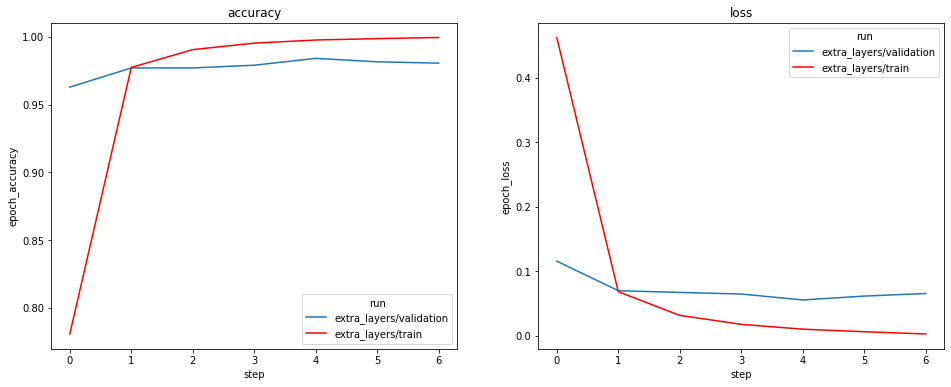
\includegraphics[width=15cm]{kapitel5/complexmodel_.png}
    \caption[Auswirkung der zusätzlichen Schichten]{Das Modell \enquote{lernt schnell} und passt sich früh an die Daten an.}
    \label{extrlayerspic}
\end{figure}

\section{Speichern und Konvertierung des Modells und der Tokens}
Das Keras Modell wird als h5-Datei gespeichert. Diese Datei kann mit dem TensorFlow.js Konverter, welches Keras Modelle in für TensorFlow.js geeignete Modelle umwandelt, konvertiert werden. Das Ergebnis dieser Umwandlung ist, eine JSON-Datei \texttt{model.json}, welches das Modell beschreibt. Dazu kommen Binäre Dateien, welches die Gewichte des Modells sind. Zusammen können Sie für Inferenz im Web mit TensorFlow.js benutzt werden. Neben dem Modell werden alle Tokens mit ihrem Index als JSON gespeichert \texttt{vocab.json} und \texttt{tokenizer.json}. Die \texttt{vocab.json} und \texttt{tokenizer.json} sind Tabellen, die jedem Token aus dem Wortschatz einen entsprechenden Index geben. Diese beide Dateien sind notwendig um mit dem Modell zu kommunizieren. Da dieses Modells keine String aufnehmen kann, wird durch diese Dateien \enquote{synthetisch} ein Vektor aus den Strings erstellt und diese werden erst dem Modell eingeführt.